\begin{frame}{2. L'apprentissage supervisé}
  \begin{itemize}
  \item Utilise des données \textit{labélisées}
  \item La machine apprend par l'exemple
  \item \textit{Prédis} le résultat pour de nouveaux événements
  \item Problèmes de régression et de classification
  \item Regression linéaire et logistique
  \item Réseaux de Neurones
  \item Arbres de décisions
  \end{itemize}
\end{frame}

\begin{frame}{2.1 La regression linéaire}
  \begin{itemize}
    
  \item Déterminer une relation \textit{linéaire} entre \textit{input(s)} (features) et \textit{output}:
    \begin{center}
      \normalsize
      \boldmath $\Rightarrow$ \unboldmath \textbf{\textcolor{orange}{Apprentissage Supervisé}}
    \end{center}
  \item Prédiction d'une valeur \textbf{continue} (e.g. non discrète, non catégorielle)
  \item Applications:
    \begin{itemize}
      \normalsize
    \item Recherche de corrélations
    \item En science, modélisation de phénomènes (physiques, biologiques, ...)
    \item Dans le domaine médical: les études épidémiologique
    \item Dans la finance/économie: prédictions des tendances
    \item $\dots$
    \end{itemize}
  \end{itemize}
  \begin{center}
    \textbf{Sujet Data Science} \boldmath $\Rightarrow$ \unboldmath \textbf{Premier algorithme à tester!}
  \end{center}
\end{frame}

\begin{frame}{2.1 Un exemple: le prix d'une carte graphique}
  \begin{itemize}
  \item La propriété principale d'une carte Graphique: valeur de \textbf{GPU}
    \vspace{0.2cm}
  \item Données, liste de carte graphiques dont on connait le couple $\{GPU;prix\}$:
  \end{itemize}

  \begin{figure}
    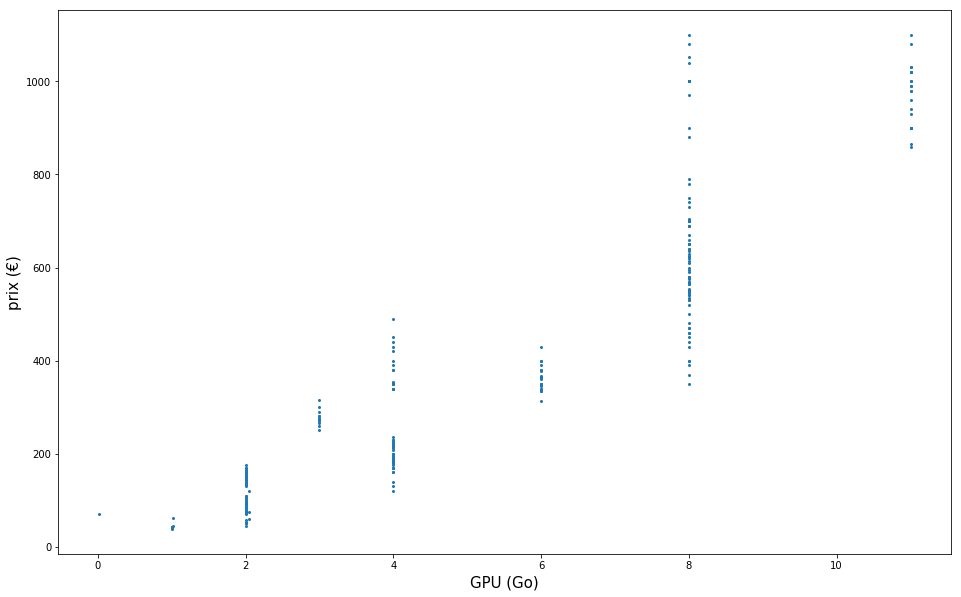
\includegraphics[width=0.6\textwidth]{figs/gpuPrices.png}    
  \end{figure}
\end{frame}

\begin{frame}{2.1 Construire un modèle (regression linéaire)}
  \begin{itemize}
  \item Soit: $x_{1}$ la valeur de GPU de nos $m$ carte graphiques, et $y$ leur prix
    \vspace{0.2cm}
  \item On cherche à déterminer le modèle pour prédire un prix $\hat{y}$ à partir $x_{1}$:
    \begin{equation*}
      \hat{y} = h_{\theta}(x_{1})
    \end{equation*}
  \item On défini le paramètre $\theta_{1}$ qui va \textit{lier} $x_{1}$ à $\hat{y}$:
    \begin{equation*}
      h_{\theta}(x) = \theta_{1} x_{1}
    \end{equation*}
  \item Rappel math: \textbf{fonction linéaire} $f(x) = kx$
  \end{itemize}
\end{frame}

\begin{frame}{2.1 Construire un modèle (regression linéaire)}
  \begin{itemize}
  \item Initialisons aléatoirement la valeur de $\theta_{1}$
  \end{itemize}
  \vspace{-0.5cm}
  \begin{figure}
    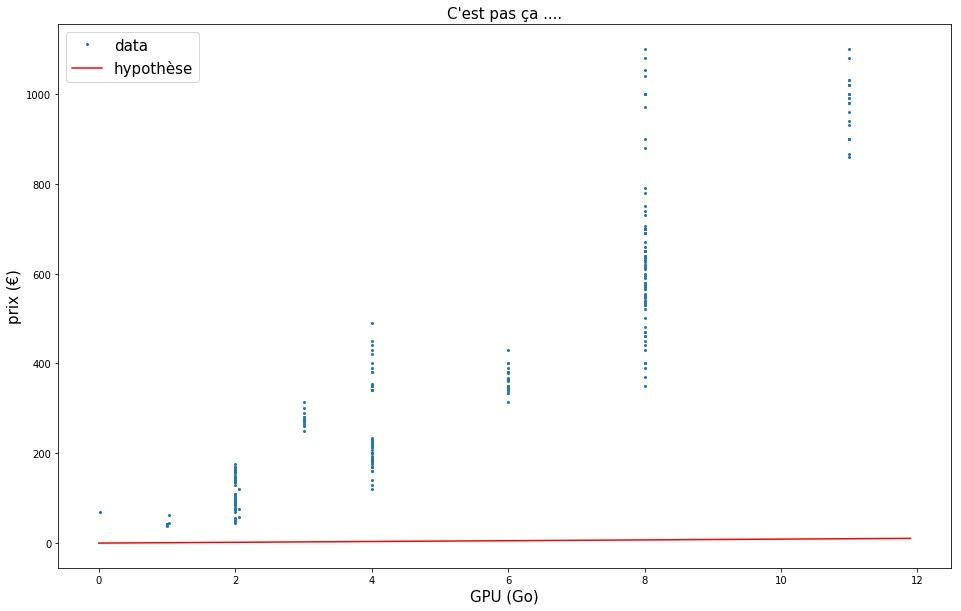
\includegraphics[width=0.6\textwidth]{figs/model.png}
  \end{figure}
  \vspace{-0.5cm}
  \begin{itemize}
  \item C'est pas encore ça ...
  \end{itemize}
\end{frame}

\begin{frame}{2.1 La fonction de coût}
  \begin{itemize}
  \item  $J(\theta)$: \textit{véracité} de notre modèle
  \item Ex, somme quadratique des erreurs: $J(\theta) = \frac{1}{2m} \displaystyle\sum_{i=0}^{m}(\hat{y}^{(i)} - y^{(i)})^{2}$
  \end{itemize}
  \begin{figure}
    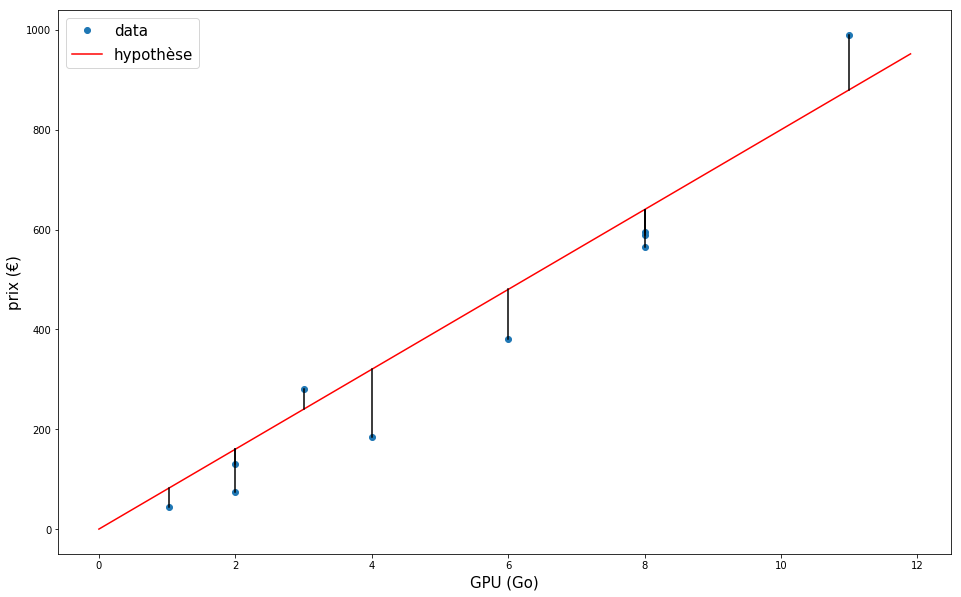
\includegraphics[width=0.6\textwidth]{figs/modelEstimation.png}
  \end{figure}  
\end{frame}

\begin{frame}{2.1 La fonction de coût}
  \begin{itemize}
  \item On cherche à trouver la valeur de $\theta_{1}$ qui \textbf{minimise} $J(\theta)$
    \vspace{0.2cm}
  \item En Brute ...
  \end{itemize}
  \vspace{-0.5cm}
  \begin{figure}
    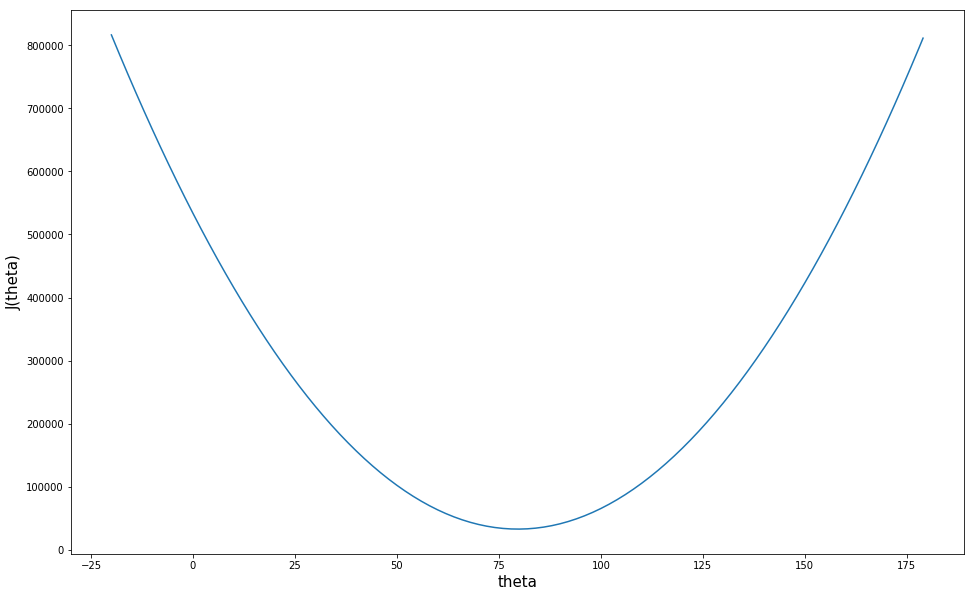
\includegraphics[width=0.6\textwidth]{figs/costFct.png}
  \end{figure}
  \vspace{-0.5cm}
  \begin{itemize}
  \item ... essayons d'optimiser
  \end{itemize}
\end{frame}

\begin{frame}{2.1 La descente de gradient}
  \begin{itemize}
  \item Algorithme pour arriver ``\textit{rapidement}'' au minimum de $J(\theta)$ 
    \vspace{0.2cm}
  \item On va utiliser la \textit{dérivation}: $\frac{d}{d\theta_{1}}J(\theta)$:
  \end{itemize}
  \begin{center}
    Si $J(\theta)$ est croissant: $\frac{d}{d\theta_{1}}J(\theta) > 0$, \hspace{0.5cm}
    Si $J(\theta)$ est décroissant: $\frac{d}{d\theta_{1}}J(\theta) < 0$
  \end{center}
  \vspace{-0.5cm}
  \begin{figure}
    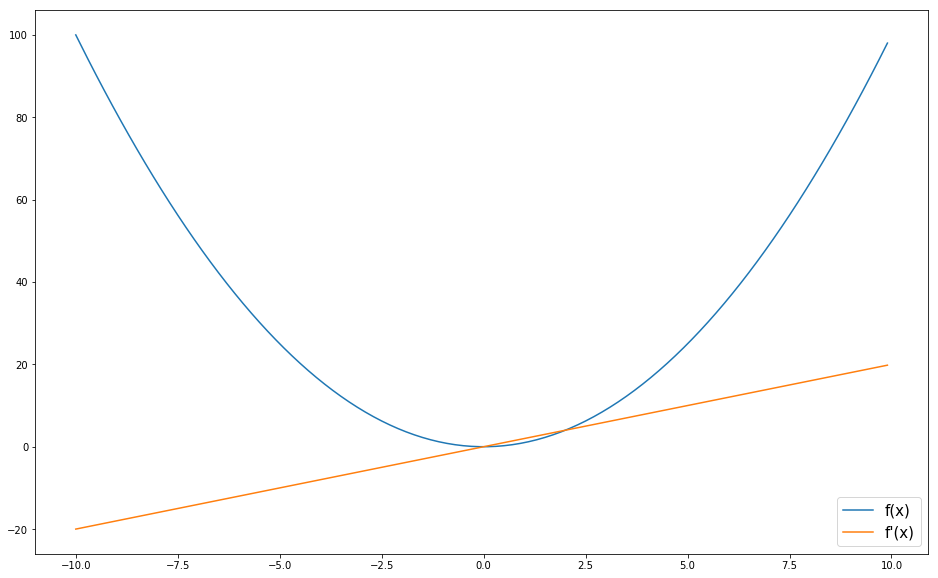
\includegraphics[width=0.5\textwidth]{figs/derivation.png}
  \end{figure}
  \vspace{-0.5cm}
\end{frame}

  
\begin{frame}{2.1 La descente de gradient}
  \begin{itemize}
  \item (Encore) un peu de math, la descente de gradient s'écrit:
  \end{itemize}
  \begin{beamerboxesrounded}[scheme=suppervise,width=\textwidth]{\textcolor{black}{Descente de gradient}}    
    \vspace{-0.2cm}
    \begin{equation*}
      \begin{matrix} \text{Répéter jusqu'à convergence:} & \{ & \\ & & \theta_{1} := \theta_{1} - \alpha \frac{d}{d\theta_{1}}J(\theta) \\ & \} & \end{matrix}
    \end{equation*}
    \vspace{-0.2cm}
    \end{beamerboxesrounded}
    \begin{itemize}
    \item $\alpha$: taux d'apprentissage (\textit{learning rate}), \textbf{seul} paramètre de l'algorithme.
      \vspace{0.2cm}
    \item On va itérativement modifier la valeur de $\theta_{1}$ en fonction de la dérivée de $J(\theta)$, jusqu'à minimiser $J(\theta)$ (\textit{convergence}).
    \end{itemize}
\end{frame}

\begin{frame}{2.1 La descente de gradient}
  \begin{itemize}
  \item Dérivons donc notre fonction de coût:
  \end{itemize}
  \begin{equation*}
    J(\theta) = \frac{1}{2m} \displaystyle\sum_{i=0}^{m}(\hat{y}^{(i)} - y^{(i)})^{2} = \frac{1}{2m} \displaystyle\sum_{i=0}^{m}(\theta_{1}x_{1}^{(i)} - y^{(i)})^{2}
  \end{equation*}
  \begin{equation*}
      \frac{d}{d\theta_{1}}J(\theta) = \frac{1}{m}\displaystyle\sum_{i=0}^{m}(\hat{y}^{(i)} - y^{(i)}) x_{1}^{(i)}
  \end{equation*}
  \begin{itemize}
  \item Un peu de \textit{hand-tunning}:
    \begin{itemize}
      \normalsize
    \item Le learning rate ($\alpha$) est fixé à $0.03$ ($0.045$ pour la démo)
    \item Précision $\epsilon = 0.0001$ pour arrêter la descente de gradient 
    \end{itemize}
  \end{itemize}
\end{frame}

\begin{frame}{2.1 Préparation du dataset}
  \begin{itemize}
  \item On sépare les données en trois sous-échantillons:
    \begin{itemize}
      \normalsize
    \item \textbf{Train:} (60$\%$) échantillon d'entrainement
    \item \textbf{Validation:} (20$\%$) échantillon qui nous permet de mesurer les performances de différents algorithmes et pour différentes valeurs d'hyperparamètres
    \item \textbf{Test:} (20$\%$) échantillon de test qui donne la performance du modèle final
    \end{itemize}
  \item On peut utiliser deux échantillons train/test (80/20 ou 70/30) dans certains cas.
  \item Il est important de séparer les données en différents sous-échantillons de test pour être sûr que le modèle de généralise bien
  \item S'assurer que les sous-échantillons proviennent de la même source et soient représentatifs
  \end{itemize}
\end{frame}

\begin{frame}{2.1 C'est parti !}
  \begin{figure}
    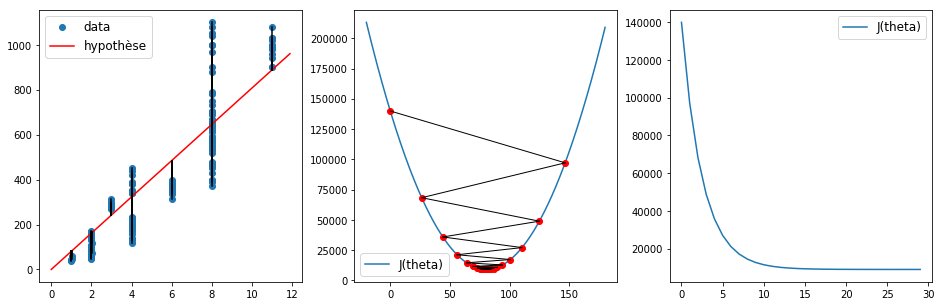
\includegraphics[width=\textwidth]{figs/gradDescent.png}
  \end{figure}
  \begin{itemize}
  \item La descente de gradient c'est achevée au bout de quelques itérations
  \item On peut voir que $J(\theta)$ a continuellement diminué à chaque itération
  \end{itemize}
  \begin{center}
    $\theta_{1} ~ \approx ~ 80$ \\
    $err_{train} ~ \approx ~ err_{test}$
  \end{center}
\end{frame}

\begin{frame}{2.1 On peut maintenant faire une prédiction}
  \begin{itemize}
  \item Quel serait le prix de cartes avec 5, 10 et 14 Go de GPU? 
  \end{itemize}
  \vspace{-0.2cm}
  \begin{figure}
    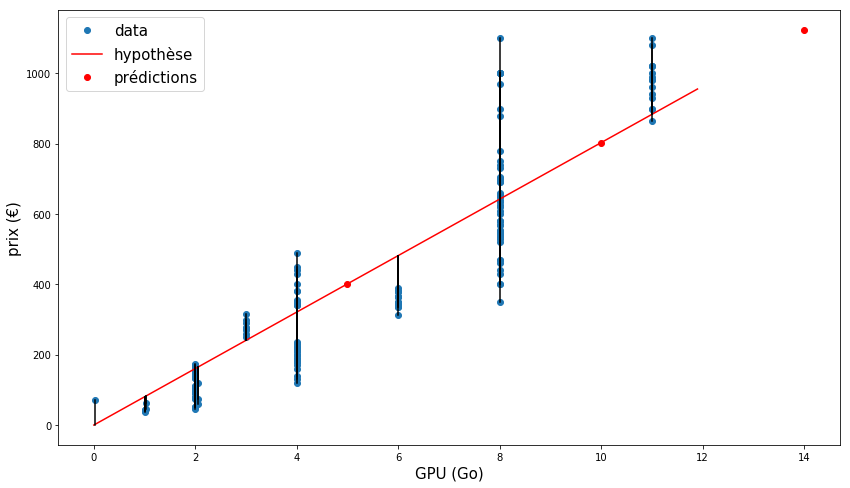
\includegraphics[width=0.6\textwidth]{figs/pred.png}
  \end{figure}
  \vspace{-0.5cm}
  \begin{itemize}
  \item On pourra les vendre autour de 400, 800 et 1100 euros!
  \end{itemize} 
\end{frame}

\begin{frame}{2.1 Le choix du taux d'apprentissage}
  \begin{itemize}
  \item \boldmath $\alpha$ \textbf{Trop grand:} la descente de gradient diverge
  \item \boldmath $\alpha$ \textbf{Trop petit:} la descente de gradient est très longue
  \end{itemize}
  \begin{figure}
    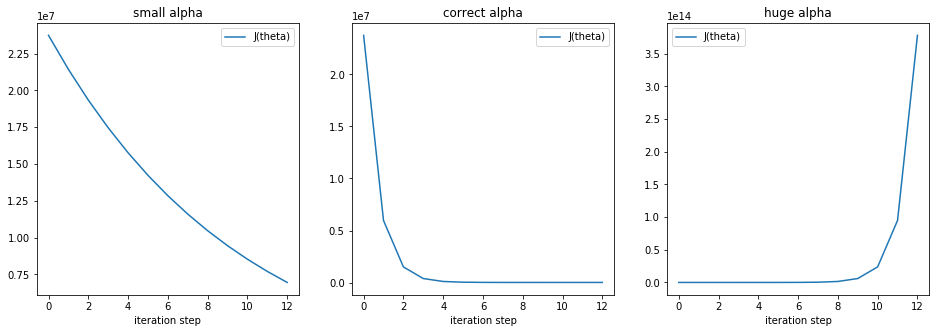
\includegraphics[width=0.9\textwidth]{figs/learningRateChoice.png}
  \end{figure}
\end{frame}

\begin{frame}{2.1 Un mot sur la regression linéaire multivariables}
  \begin{itemize}
  \item Même principe, mais avec plusieurs variables $x_{i}$ (donc plusieurs paramètres $\theta_{i}$)
  \item on peut rajouter un biais $\theta_{0}$, cad un terme constant: $\hat{y} = \theta_{0} + \theta_{1}x_{1} + \dots$
  \item Notre fonction hypothèse s'écrie alors:
  \end{itemize}
  \begin{equation*}
    h_{\theta}(x) = \theta_{0} + \theta_{1}x_{1} + \theta_{2}x_{2} + \dots + \theta_{n}x_{n} = \theta_{0} + \displaystyle\sum_{i=1}^{n} \theta_{i} x_{i}
  \end{equation*}
  \begin{itemize}
    \item \textbf{\textcolor{orange}{Astuce:}} On définit $x_{0} = 1$, et on re-écrit la fonction hypothèse:
  \end{itemize}
  \begin{equation*}
    h_{\theta}(x) = \theta_{0}x_{0} + \theta_{1}x_{1} \dots + \theta_{n}x_{n} = \displaystyle\sum_{i=0}^{n} \theta_{i} x_{i}
  \end{equation*}

  \begin{itemize}
  \item La fonction de coût reste inchangée
  \end{itemize}
\end{frame}

\begin{frame}{2.1 Un mot sur la regression linéaire multivariables}
  \begin{itemize}
  \item Dans le cas multivariables, la descente de gradient devient:
  \end{itemize}
    \begin{beamerboxesrounded}[scheme=suppervise,width=\textwidth]{\textcolor{black}{Descente de gradient (cas multivariables)}}    
    \vspace{-0.2cm}
    \begin{equation*}
      \begin{matrix} \text{Répéter jusqu'à convergence:} & \{ & \\
        & & \theta_{0} := \theta_{0} - \alpha \frac{d}{d\theta_{0}}J(\theta) \\
        & & \theta_{1} := \theta_{1} - \alpha \frac{d}{d\theta_{1}}J(\theta) \\
        & & \theta_{2} := \theta_{2} - \alpha \frac{d}{d\theta_{2}}J(\theta) \\
        & & \dots \\
        & \} & \end{matrix}
    \end{equation*}
    \vspace{-0.2cm}
  \end{beamerboxesrounded}
    \begin{itemize}
    \item Il est très important de simultanément changer les valeurs des paramètres.
    \end{itemize}
\end{frame}

\begin{frame}{2.1 Un mot sur la regression linéaire multivariables}
  \begin{itemize}
  \item Pour illustrer: régression linéaire à deux dimensions
  \end{itemize}
  \begin{figure}
    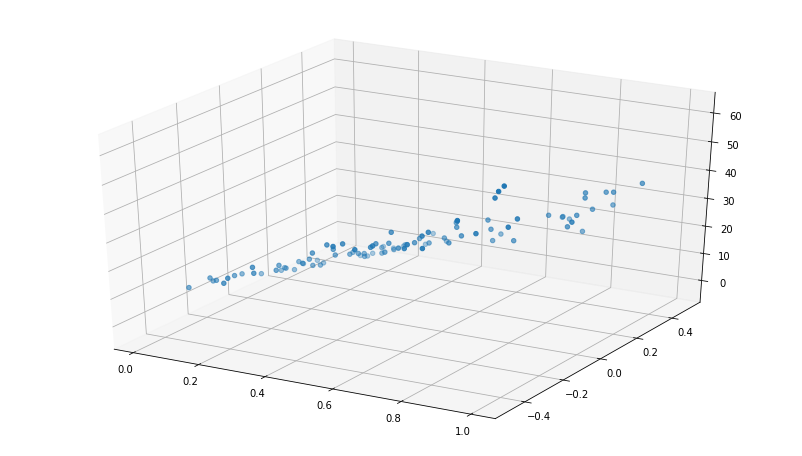
\includegraphics[width=0.4\textwidth]{figs/multiVarData.png}
    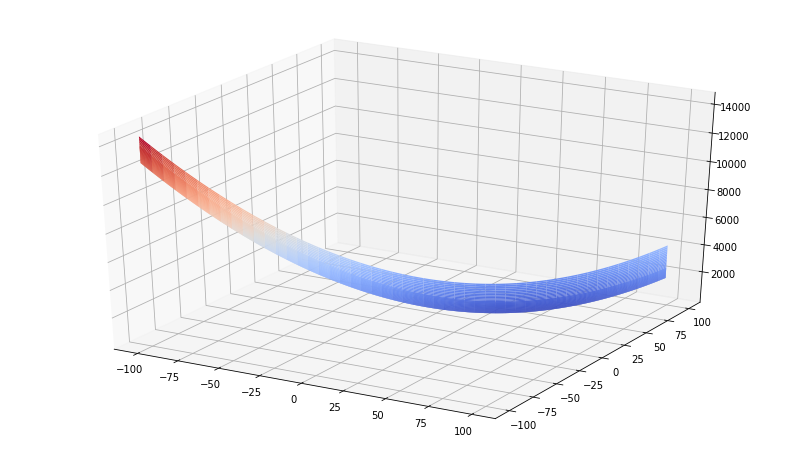
\includegraphics[width=0.4\textwidth]{figs/multiVarCostFct.png}\\
    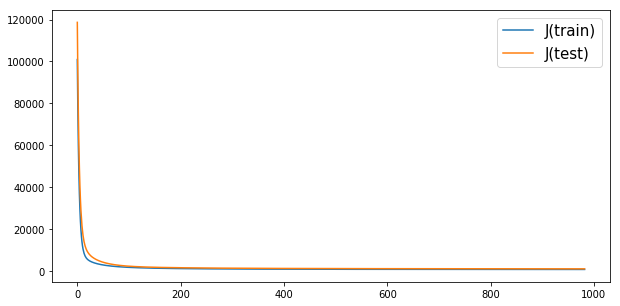
\includegraphics[width=0.45\textwidth]{figs/multiVarDesc.png}
  \end{figure}
\end{frame}

\begin{frame}{2.1 Affinons notre modèle de carte graphiques}
  \begin{itemize}
  \item Plus de features: chipset, fréquence, consommation, ...
  \item Il va falloir explorer et nettoyer les données:
    \begin{itemize}
      \normalsize
    \item Gestion des données manquantes / abbérantes
    \item \textit{Features engineering}
    \item Normaliser le dataset (pour accélérer la descente de gradient)
    \end{itemize}
  \end{itemize}
\end{frame}

\begin{frame}{2.1 Features scaling}
  \begin{itemize}
  \item Mettre les variables à la même échelle (performances)
  \item Normaliser les variables: $-1 \leq x_{i} \leq 1$
  \end{itemize}
  \vspace{-0.2cm}
  \begin{table}
    \footnotesize
        {\def\arraystretch{2}\tabcolsep=8pt
          \begin{tabular}{l|l|l}
            & \textbf{Feature Scaling} & \textbf{Mean normalization}\\
            \hline
            \textbf{Start range} & $x_{min} \leq x \leq x_{max}$ & $x_{min} \leq x \leq x_{max}$ \\
            \textbf{Transformation} & $x := \frac{x - x_{min}}{x_{max} - x_{min}}$ & $x := x - x_{mean}$ \\
            \textbf{New range} & $0 \leq x \leq 1$ & $(x_{min}-x_{mean}) \leq x \leq (x_{max}-x_{mean})$
          \end{tabular}
        }
  \end{table}
  \vspace{-0.2cm}
  \begin{itemize}
  \item En combinant les deux: \boldmath \textcolor{orange}{$x := \frac{x - x_{mean}}{x_{max} - x_{min}}$} $\Rightarrow$ \textcolor{orange}{$-1 \leq x \leq 1$} 
    \vspace{0.2cm}
    \footnotesize
  \item\textbf{Remarque:} Il est possible de remplacer $x_{max} - x_{min}$ par l'écart type: $\sigma_{x} = \sqrt{\frac{1}{n}\displaystyle\sum_{i=1}^{n}(x_{i} - \bar{x})^{2}}$
  \end{itemize}
\end{frame}

\begin{frame}{2.1 Régression linéaire multivariables: Résultats}
  \begin{itemize}
  \item On utilise la même valeur de $\epsilon = 0.0001$ et $\alpha = 0.03$
  \item Plus long! Mais meilleur résultats:
  \item Modèle simple: $err ~ \approx ~ 100$
  \item Modèle multivariable: $err ~ \approx ~ 30$
  \end{itemize}
  \begin{figure}
    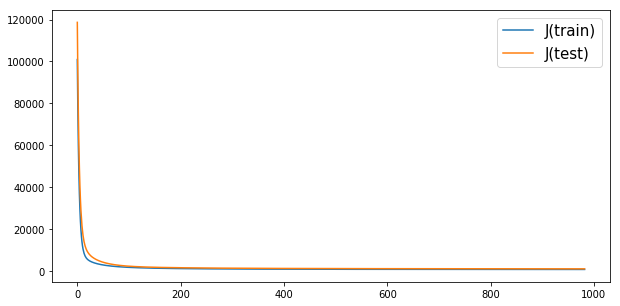
\includegraphics[width=0.45\textwidth]{figs/multiVarDesc.png}\\
  \end{figure}
\end{frame}
  
\begin{frame}{2.1 Pour conclure sur la régression linéaire}
  \begin{itemize}
  \item \textbf{Regression Linéaire:} $\hat{y}$ est une valeur \textit{continue}
    \begin{itemize}
      \normalsize
    \item Valeur discrète: \textbf{Regression Logistique} (\textit{classification})
    \end{itemize}
    \vspace{0.2cm}
  \item Le résultat $\hat{y}$ dépend \textbf{linéairement} des variables $x_{i}$ si:
    \begin{equation*}
      \hat{y} = \theta_{1}x_{1} + \dots + \theta_{n}x_{n} = \displaystyle\sum_{i=1}^{n} \theta_{i} x_{i}
    \end{equation*}
  \item \textbf{Supervisé}: $y$ connu pour chaque élément du le jeu de données d'entrainement
  \item Facile à implémenter (encore plus avec Scikit-learn ...), rapide: 
  \end{itemize}
  \begin{center}
    $\Rightarrow$ bon point de départ sur un sujet
  \end{center}
\end{frame}

\begin{frame}{2.2 La régression logistique}
  \begin{itemize}
  \item \textbf{\textcolor{orange}{Classification}}: prédire un nombre limités de valeurs discrètes
    \begin{itemize}
    \item \textbf{Classification binaire}: Deux valeurs possibles: Vrai ou Faux (spam / non spam)
    \item \textbf{Classification multiclasse}: plusieurs valeurs possibles (camion, voiture, piétons, vélos, ...)
    \end{itemize}
    \vspace{0.5cm}
  \item \textcolor{orange}{\textbf{Classification binaire:}} En utilisant la régression linaire?
    \begin{itemize}
    \item $y \in \{0,1\}$ \textcolor{orange}{$\Rightarrow$} On défini un seuil $S$ pour $h_{\theta}(x)$:
      \begin{equation*}
        \begin{cases}
          h_{\theta}(x) \geq S \rightarrow y = 1\\
          h_{\theta}(x) < S \rightarrow y = 0
        \end{cases}
      \end{equation*}
    \end{itemize}
  \item \textbf{Problème:} On voudrait que $0 \leq h_{\theta}(x) \leq 1$
  \end{itemize}
  \begin{center}
    $\Rightarrow$ Il faut redéfinir notre fonction hypothèse!
  \end{center}
\end{frame}

\begin{frame}{2.2 La régression logistique}
  \begin{itemize}
  \item Modèle de la régression logistique:
    \begin{itemize}
      \item On utilise la \textbf{Fonction Sigmoïde} $g(z)=\frac{1}{1+e^{-z}}$
    \end{itemize}
  \end{itemize}
  \begin{minipage}{0.4\textwidth}
    \begin{equation*}
      \begin{cases}
        z = \displaystyle\sum_{i=0}^{n} \theta_{i} x_{i}\\
        h_\theta(x) = g(z) \\
      \end{cases}
    \end{equation*}
    \vfill
    \begin{equation*}
      \textcolor{blue}{0 \leq h_{\theta}(x) \leq 1}
    \end{equation*}
  \end{minipage}
  \begin{minipage}{0.5\textwidth}
    \begin{figure}
      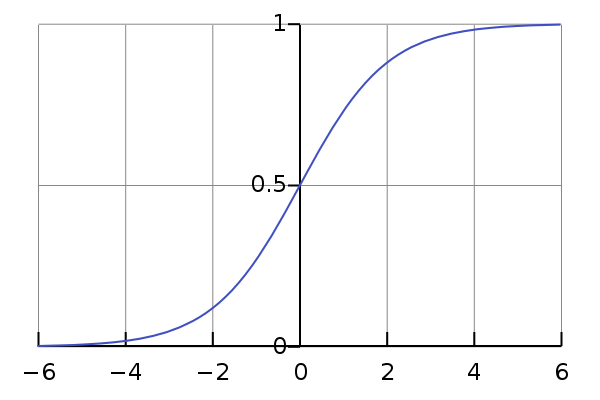
\includegraphics[width=0.9\textwidth]{figs/logisticFct.png}
    \end{figure}
    \begin{center}
      \tiny
      \vspace{-0.5cm}
      \textcolor{blue}{$g(z)$} depuis \href{https://en.wikipedia.org/wiki/Sigmoid_function}{\color{blue}{Wikipedia}}
    \end{center}
  \end{minipage}
  \vfill
  \begin{itemize}
  \item \textbf{Classification:} On prédit une \textbf{probabilité}
  \end{itemize}
\end{frame}

\begin{frame}{2.2 La régression logistique}
  \begin{itemize}
  \item On change également la fonction de coût:
  \end{itemize}
  \begin{equation*}
    J(\theta)=\frac{1}{m} \displaystyle \sum_{i=1}^{m}Cost(h_{\theta}(x^{(i)}),y^{(i)})
  \end{equation*}
  \begin{itemize}
  \item Avec:
  \end{itemize}
  \begin{equation*}
    Cost(h_{\theta}(x),y) = 
    \begin{cases}
      -log(h_{\theta}(x)) & \quad \text{if } y = 1 \\
      -log(1 - h_{\theta}(x)) & \quad \text{if } y = 0 \\
    \end{cases}
  \end{equation*}
  \begin{figure}
    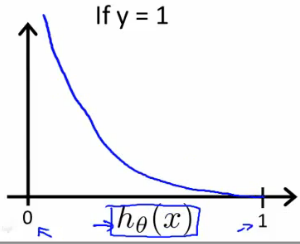
\includegraphics[width=.22\textwidth]{figs/logisticRegressionCostFunction1.png}
    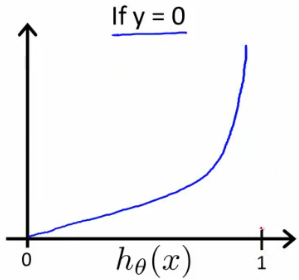
\includegraphics[width=.2\textwidth]{figs/logisticRegressionCostFunction2.png}
  \end{figure}
\end{frame}

\begin{frame}{2.2 La régression logistique}
  \begin{itemize}
  \item Et la \textcolor{orange}{\textbf{Classification multiclasse}} ? $y \in \{0,1,2,\dots,n\}$
  \item La \textbf{descente de gradient} ne permet pas de la résoudre
  \item On peut \textit{tricher} en utilisant la méthode \textit{'One-vs-all'}:
    \begin{itemize}
    \item On remplace le problème multiclasse par $n+1$ problèmes binaire
    \item Probabilité que $y$ soit dans une classe ou qu'il soit dans une des autres:
    \end{itemize}
  \end{itemize}
  \begin{equation*}
    \begin{cases}
      h_{\theta}^{(0)} = P(y=0 | x;0)\\
      h_{\theta}^{(1)} = P(y=1 | x;0)\\
      \dots \\
      h_{\theta}^{(n)} = P(y=n | x;0)\\
      \text{prediction} = max_{i}(h_{\theta}^{(i)}(x))\\
    \end{cases}
  \end{equation*}
  \begin{itemize}
  \item Algorithme d'optimisation avancés: \textit{Conjugate gradient}, \textit{(L-)BFGS}, $\dots$
  \end{itemize}
\end{frame}

\begin{frame}{2.2 La régression logistique}
  \begin{itemize}
  \item Application: vision par ordinateur, reconnaissance d'images.
  \item Objets \textit{"simples"}: chiffres manuscrits
  \item Régression logistique multiclasse sur MNIST:
    \begin{itemize}
      \normalsize
    \item Durée d'apprentissage $\sim 20 sec$ $~/~$ Précision $\approx 91\%$
    \end{itemize}
  \end{itemize}
  \vfill
  \begin{minipage}{0.45\textwidth}
    \begin{figure}
      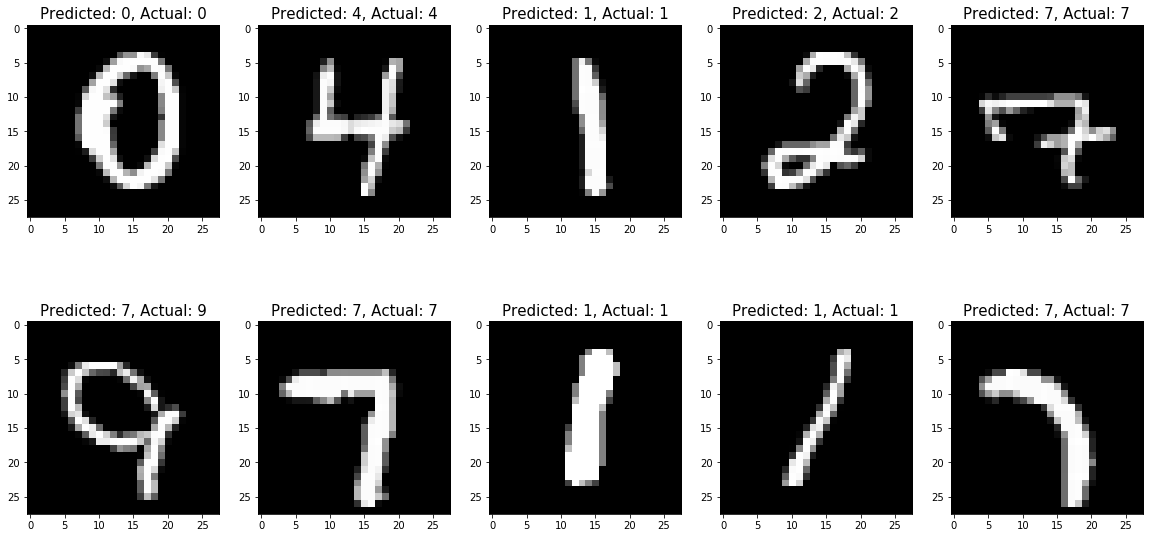
\includegraphics[height=0.37\textheight]{figs/digitReco_regrLog.png}
    \end{figure}
  \end{minipage}
  \hfill
  \begin{minipage}{0.45\textwidth}
    \begin{figure}
      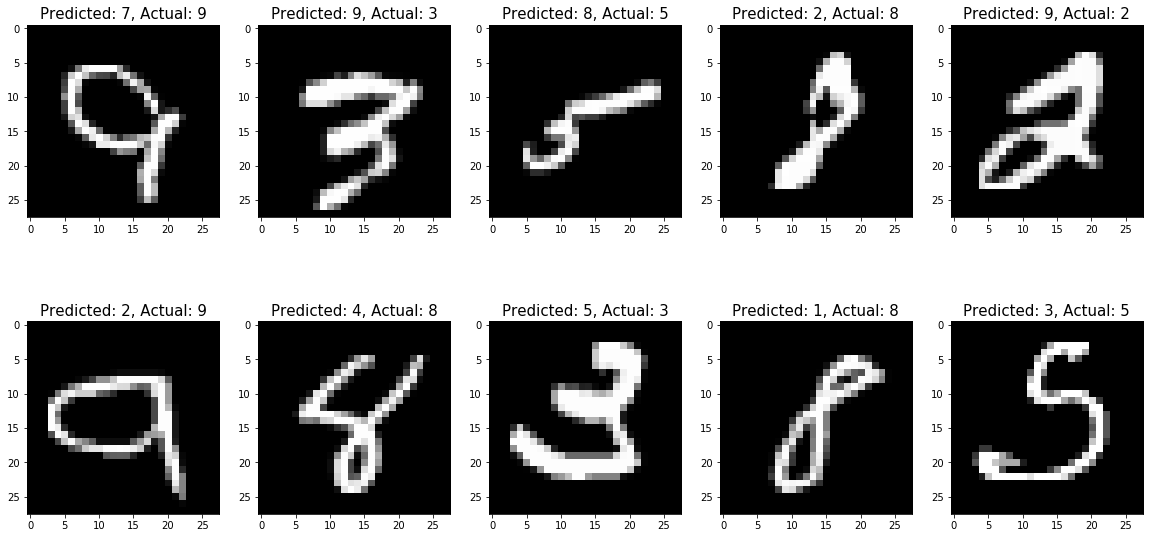
\includegraphics[height=0.37\textheight]{figs/bad_digitReco_regrLog.png}
    \end{figure}
  \end{minipage}
\end{frame}

\begin{frame}{2.3 Les problèmes de biais et de variance}
  \begin{figure}
    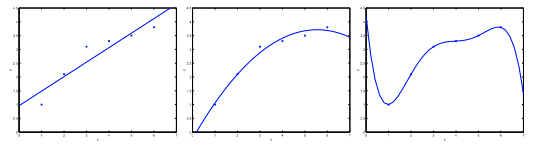
\includegraphics[width=0.9\textwidth]{figs/theProblemOfOverfitting.png}
  \end{figure}
  \footnotesize
  \vspace{-1cm}
  \begin{center}
    \textit{Underfitting} (Bias) \hspace{1.5cm} \textit{Just fine!} \hspace{1.5cm} \textit{Overfitting} (Variance)
  \end{center}
  \begin{itemize}
  \item \textbf{Underfitting}: modèle trop simple (pas assez de variables)
  \item \textbf{Overfitting}: modèle trop complexe, deux manière de résoudre:
    \begin{itemize}
    \item Réduire le nombres de variables ou changer les paramètres du modèle
    \item Utiliser des méthodes de \textbf{régularisation}
    \end{itemize}
  \end{itemize}  
\end{frame}

\begin{frame}{2.3 Les bonnes pratiques: biais et variance}
  \begin{itemize}
  \item Si $J_{train}(W,b) >> J_{valid}(W,b)$: problème de variance: \textbf{Overfitting}
  \item Si $J_{train}(W,b) \approx J_{valid}(W,b) >> 0$: problème de biais: \textbf{Underfitting}
  \item Comment diagnostiquer? deux valeurs à regarder:
    \begin{itemize}
      \normalsize
    \item Erreur de l'échantillon d'entrainement: $t_{err}$
    \item Erreur de l'échantillon de validation: $v_{err}$
    \end{itemize}
  \item On estime le cas idéal (Bayes ou opérateur humain): $\approx 0\%$
  \end{itemize}
  \vspace{0.5cm}
  \begin{minipage}{.39\textwidth}
    \begin{figure}
      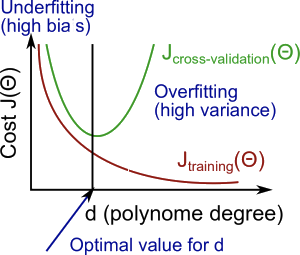
\includegraphics[trim={0 54 0 0},clip,width=\textwidth]{figs/biasVsVariance}
    \end{figure}
    \vspace{-0.5cm}
    \begin{center}
      \scriptsize
      \href{https://www.coursera.org/learn/machine-learning}{\color{blue}{[Coursera]}}
    \end{center}
  \end{minipage}
  \begin{minipage}{.59\textwidth}
    \begin{table}
      \begin{tabular}{l|l|l}
        $t_{err}$ & $v_{err}$ & problème \\
        \hline
        1$\%$ & 11$\%$ & haute variance \\
        15$\%$ & 16$\%$ & haut biais \\
        15$\%$ & 30$\%$ & haut biais \& haute variance \\
        0.5$\%$ & 1$\%$ & bas biais \& basse variance \\
      \end{tabular}
    \end{table}
  \end{minipage}
\end{frame}

\begin{frame}{2.3 Les bonnes pratiques: courbes d'apprentissage}
  \begin{itemize}
  \item Entrainer un modèle en augmentant le nombre d'exemples et monitorer l'évolution de l'erreur:
  \end{itemize}
  \begin{figure}
    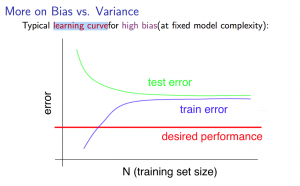
\includegraphics[trim = {0 0 0 32}, clip, width=0.44\textwidth]{figs/learningCurves1.png}
    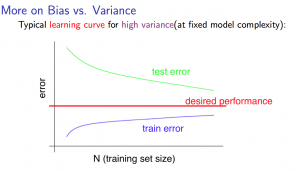
\includegraphics[trim = {0 0 0 30}, clip, width=0.48\textwidth]{figs/learningCurves2.png}
  \end{figure}
  \vspace{-0.5cm}
  \begin{center}
    \scriptsize
    Biais et variance \href{https://www.coursera.org/learn/machine-learning}{\color{blue}{[Coursera]}}
  \end{center}  
\end{frame}

\begin{frame}{2.3 Les bonnes pratiques: Que faire?}
  \begin{table}
    \footnotesize
    \begin{tabular}{ccccl}
      \multicolumn{3}{l}{\textcolor{orange}{\textbf{$\bullet$ Haut Biais?}}} & \boldmath $\rightarrow$ \textbf{Oui} $\rightarrow$ \unboldmath & Changer les hyperparamètres \\
      \multicolumn{3}{l}{(Performance entrainement)} & & Plus de données et étude qualitée \\
      & & & & Algorithme plus complexe \\
      & & \boldmath $\downarrow$ \unboldmath & & \multicolumn{1}{c}{\boldmath $\downarrow$ \boldmath} \\
      & & \textbf{Non} & & \multicolumn{1}{c}{\textit{\textcolor{orange}{Recommencer!}} \boldmath $\rightarrow$ \unboldmath}\\
      & & \boldmath $\downarrow$ \unboldmath & & \\
      & & & & \\
      \multicolumn{3}{l}{\textcolor{orange}{\textbf{$\bullet$ Haute Variance?}}} & \boldmath $\rightarrow$ \textbf{Oui} $\rightarrow$ \unboldmath & Changer les hyperparamètres \\
      \multicolumn{3}{l}{(Performance validation)} & & Plus de données et étude qualitée  \\
      & & & & Régularisation \\
      & & \boldmath $\downarrow$ \unboldmath & & \multicolumn{1}{c}{\boldmath $\downarrow$ \boldmath} \\
      & & \textbf{Non} & & \multicolumn{1}{c}{\textit{\textcolor{orange}{Recommencer!}} \boldmath $\rightarrow$ \unboldmath}\\
      & & \boldmath $\downarrow$ \unboldmath & & \\
      & & & & \\
      & & \textcolor{orange}{\textbf{OK!}} & & \\      
    \end{tabular}
  \end{table}
\end{frame}

\begin{frame}{2.3 La régularisation}
  \begin{itemize}
  \item Contraindre les paramètres $\theta_{j}$ sans réduire le nombre de variables
  \item On ré-écrit la fonction de coût avec le \textcolor{blue}{terme de régularisation}:
  \end{itemize}
  \begin{equation*}
    J(\theta) = \frac{1}{2m}(\displaystyle\sum_{i=1}^{m}(h_{\theta}(x^{(i)}) - y^{(i)})^{2} + \textcolor{blue}{\lambda \displaystyle\sum_{j=1}^{n}\theta_{j}^{2}})
  \end{equation*}
  \begin{itemize}
  \item \boldmath $\lambda$: Paramètre de régularisation
  \item Si $\lambda$ est trop grand: risque d'\textit{underfitting}
  \item Si $\lambda = 0$: pas de régularisation. 
  \item \textbf{Remarque:} On ne régularise pas le terme constant $\theta_{0}$
  \end{itemize}
\end{frame}

\begin{frame}{2.4 Les arbres de décisions}
  \begin{itemize}
  \item Effectue une prédiction (regression ou classification) par une succession de decision simples: \textit{if-else-then} sur les différentes variables
  \item \textit{Arbre} = suite de décisions (\textit{noeuds}) ammenant à une prédiction (\textit{feuille})
  \end{itemize}
  \begin{minipage}{.45\textwidth}
    \begin{itemize}
    \item La complexité de la structure de données qu'il est possible de représenter avec une arbre de décision est proportionelle à la profondeur de l'arbre
    \end{itemize}
  \end{minipage}
  \begin{minipage}{.54\textwidth}
    \begin{figure}
      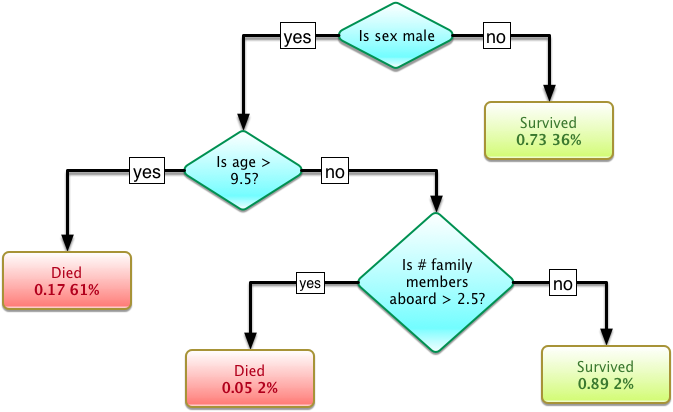
\includegraphics[width=.9\textwidth]{figs/decisionTreeExample.png}
    \end{figure}
    \begin{center}
      \scriptsize
      \textit{Un arbre pour déterminer la probabilité de survie des passagers du Titanic (depuis \href{https://en.wikipedia.org/wiki/Decision_tree_learning}{\color{blue}{Wikipedia}})}
    \end{center}
  \end{minipage}
\end{frame}

\begin{frame}{2.4 Les arbres de décisions: Apprentissage}
  \begin{itemize}
  \item La \textit{meilleure} séparation possible est déterminée:
    \begin{itemize}
      \normalsize
    \item Toutes les variables/sélection possibles
    \item Celle qui minimise une fonction de coût
    \end{itemize}
  \item L'échantillon d'entrainement est séparé suivant cette décision, créant ainsi deux feuilles (sous-échantillon)
  \item On recommence l'opération tant que l'on a pas atteint la profondeur voulue ou bien que la pureté de chaque feuille atteint un niveau satisfaisant (à déterminer)
  \end{itemize}
  \vspace{1cm}
  \textbf{Remarque:} Il est possible d'utiliser la même variables pour différents noeud.
\end{frame}

\begin{frame}{2.4 Les arbres de décisions}
  \begin{itemize}
  \item Ces algorithmes sont faciles à interpréter (et à visualiser)
  \item Tout les types de données (catégorielle, numérique, ...) peuvent être mélangés
  \end{itemize}
  \begin{figure}
    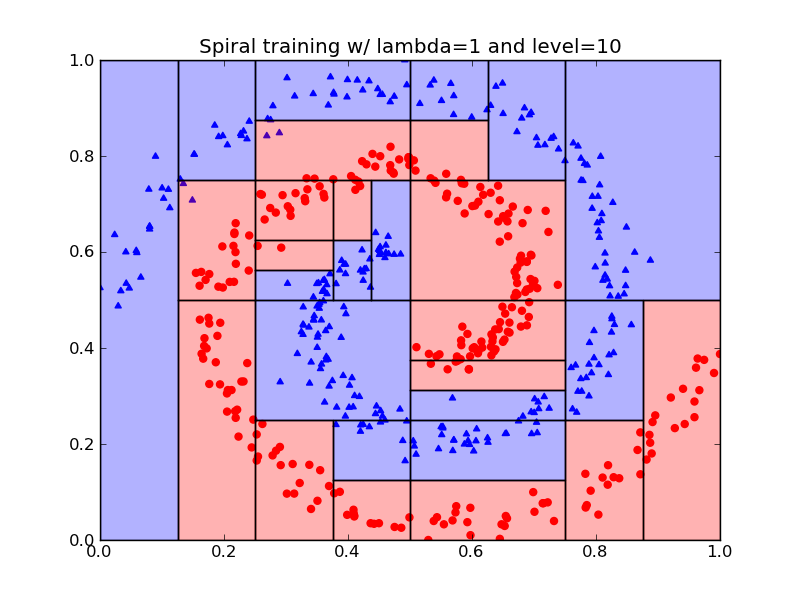
\includegraphics[trim={0 0 0 40},clip,width=.3\textwidth]{figs/spiralDTresult.png}
    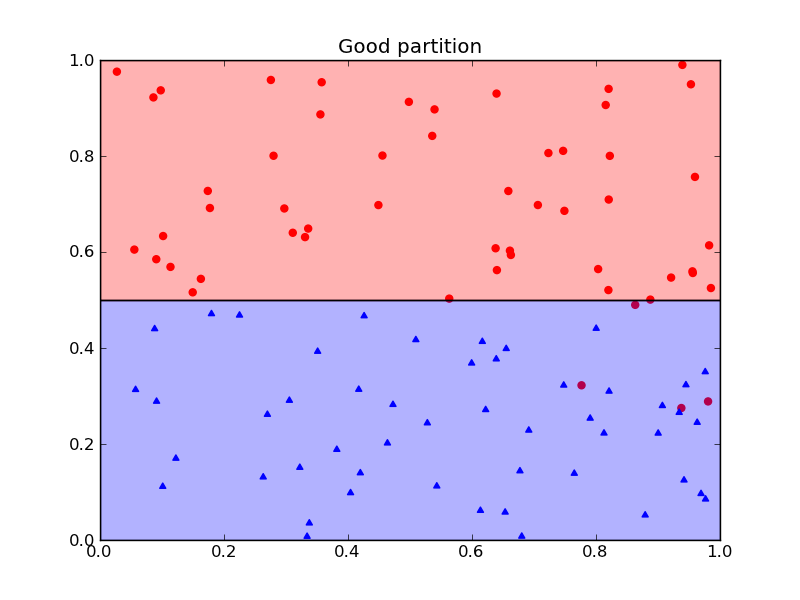
\includegraphics[trim={0 0 0 40},clip,width=.3\textwidth]{figs/goodPartitionDT.png}
    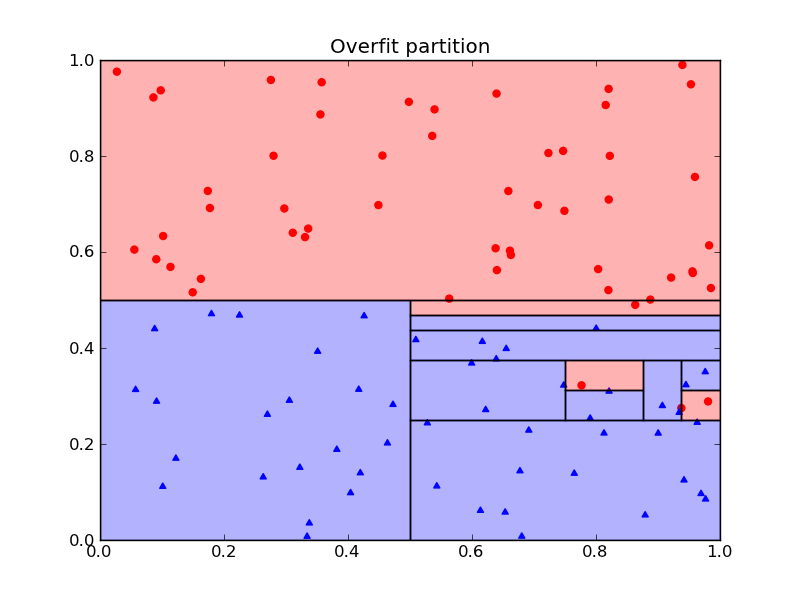
\includegraphics[trim={0 0 0 40},clip,width=.3\textwidth]{figs/overfittingPartitionDT.png}
  \end{figure}
  \vspace{-0.8cm}
  \begin{center}
    \scriptsize
    \textit{Illustration depuis \href{https://www.classes.cs.uchicago.edu/archive/2013/winter/12200-1/assignments/pa4/index.html}{\color{blue}{University of Chicago}}}
  \end{center}
  \begin{itemize}
  \item Risque d'\textit{overfitting} (sur-apprentissage) du modèle qui se généralise mal
  \item Algorithmes très sensibles au jeu de données d'entrainement
  \end{itemize}
\end{frame}

\begin{frame}{2.4 Les arbres de décisions: méthodes d'ensemble}
  \begin{itemize}
  \item Pour pallier les faiblesse des arbres de décision, on les utilise comme \textit{base learners} dans des méthodes qui en regroupe plusieurs
  \item Il existe deux familles de méthodes:
    \begin{itemize}
      \normalsize
      \vspace{0.5cm}
    \item \textbf{averaging}: plusieurs estimateurs (\textit{learners}) indépendant dont on moyenne les prédictions (\textit{Random Forests}, $\dots$)
      \vspace{0.5cm}
    \item \textbf{boosting}: plusieurs estimateurs combinés (\textit{AdaBoost}, \textit{XGBoost}, $\dots$)
    \end{itemize}
  \end{itemize}
\end{frame}

\begin{frame}{2.4 Exemple d'algorithme d'\textit{averaging}: \textbf{Random Forests}}
  \begin{itemize}
  \item \textit{Bagging}: Chaque estimateur (arbre) de l'ensemble est construit à partir d'un sous-échantillon aléatoire (avec replacement) de l'échantillon d'entrainement (\textit{Bootstrap aggregating})
  \item \textit{Features bagging}: La \textit{meilleure} séparation possible sur un sous-échantillon aléatoire des variables
  \item Soit $f_{b}$, l'arbre entrainé sur le sous-échantillons $b$ ($b \in[1,B]$), on calcule la prédiction globale en moyennant les prédictions de tout les arbres:
  \end{itemize}
  \begin{equation*}
    \hat{f} = \frac{1}{B}\displaystyle\sum_{b=1}^{B} f_{b}(x)
  \end{equation*}
  \begin{itemize}
  \item Cette méthode obtient de meilleure performance car elle réduit la \textit{variance} du modèle sans accroitre le \textit{biais}
  \end{itemize}
\end{frame}

\begin{frame}{2.4 Exemple d'algorithme de \textit{boosting}: \textbf{AdaBoost}}
  \begin{itemize}
  \item L'apprentissage d'un même \textit{learner} est répété en modifiant le jeu de données à chaque itération
  \item On utilise des poids: $w_{i}$ pour $i \in [1,N]$. Initialement: $w_{i} = 1/N$
  \item À chaque itération, le poids des exemples correctement prédits diminue tandis que celui des exemples dont les prédictions sont fausse augmente
  \item L'algorithme devient plus sensibles aux exemples difficiles à prédire
  \end{itemize}
\end{frame}

\begin{frame}{2.4 Exemple d'algorithme de \textit{boosting}: \textbf{XGBoost}}
  \begin{itemize}
  \item Obtient d'excellent résultats sur la plupart des cas d'usages (classification et régression)
  \item Des arbres sont générés aléatoirement comme pour les \textit{random forests}
  \item Mais au lieu de moyenner les prédictions, on additionne les prédictions
    \begin{itemize}
    \item À chaque étape, des arbres sont générés et on sélectionne celui qui optimise la fonction d'objectif (une fonction de coût + une fonction qui mesure la complexité du modèle)
    \item On additionne la prédiction de cet arbre à la prédiction du modèle et on recommence jusqu'à atteindre une performance suffisante
    \end{itemize}
  \end{itemize}
  \begin{equation*}
    \begin{cases}
      \hat{y_{i}}^{(0)} = 0 \\
      \hat{y_{i}}^{(1)} = \hat{y_{i}}^{(0)} + f_{1}(x_{i}) = f_{1}(x_{i})\\
      \hat{y_{i}}^{(2)} = \hat{y_{i}}^{(1)} + f_{2}(x_{i}) = f_{1}(x_{i}) + f_{2}(x_{i})\\
      \dots\\
      \hat{y_{i}}^{(t)} = \hat{y_{i}}^{(t-1)} + f_{t}(x_{i}) = \displaystyle\sum_{k=1}^{t} f_{k}(x_{i}) \\
    \end{cases}
  \end{equation*}
\end{frame}

\begin{frame}{2.4 Arbres de décision: \textit{Titanic}}
  \begin{figure}
    \includegraphics[width=\textwidth]{notebook/decisionTrees/titanic.pdf}
  \end{figure}
  \begin{table}
    \footnotesize
    \begin{tabular}{l|l|l|l|l}
      & \textbf{Decision Tree}  & \textbf{Random Forest}  & \textbf{AdaBoost}  & \textbf{XGBoost} \\
      \hline
      \textbf{Accuracy (\boldmath $\%$)} & 77.6 & 81.1 & 83.2 & 83.9 \\
    \end{tabular}
  \end{table}
\end{frame}

